\section{Métricas de Evaluación}
El objetivo de la segmentación es separar los objetos deseados del fondo para el estudio futuro~\cite{carrasco}. A partir de los objetos segmentados se pueden clasificar los píxeles en cuatro resultados posibles:
\addsymbol{symbol:VP} \addsymbol{symbol:VN} 
\addsymbol{symbol:FP} \addsymbol{symbol:FN} 
\begin{itemize}
\item Verdadero Positivo ($VP$), píxel que pertenece al objeto segmentado y es segmentado como tal.
\item Falso Positivo ($FP$), píxel que no pertenece al objeto segmentado y es segmentado como parte del mismo erróneamente.
\item Verdadero Negativo ($VN$), píxel que no pertenece al objeto segmentado y no es segmentado como parte del mismo.
\item Falso Negativo ($FN$), píxel que pertenece al objeto segmentado y no es segmentado como tal.
\end{itemize}
La clasificación de los resultados obtenidos para las distintas variables se puede observar en la Figura \ref{img:vpfp}. Las zonas en donde el objeto a segmentar y la segmentación realizada se interceptan corresponde a los píxeles considerados como $VP$, en donde el objeto no intercepta a la segmentación realizada corresponde a los $FN$. Posteriormente los píxeles que son parte de la segmentación realizada pero no el objeto son los $FP$ y los píxeles del fondo de la imagen que si corresponden al fondo son los $VN$.
\begin{figure}[H]
\centering
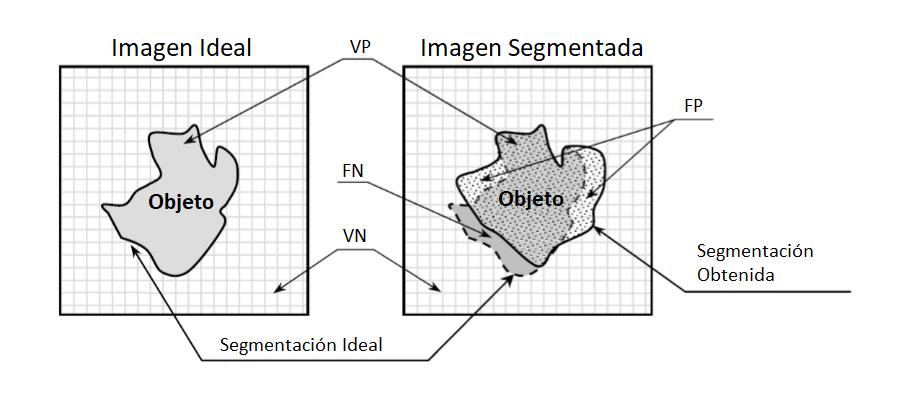
\includegraphics[width=160mm]{./imagenes/metricas-imagen.png}
\caption{Resultados posibles de la segmentación}
\label{img:vpfp}
\end{figure}
Para el problema estudiado la imagen ideal representa la segmentación hecha por un profesional, y la imagen segmentada representa la segmentación de los amastigotes obtenidos automáticamente. Se puede considerar que los $VP$ son los píxeles que pertenecen al amastigote y fueron segmentados correctamente, los $FP$ son los píxeles que fueron segmentados como parte de el amastigote pero no lo son, los $FN$ son los píxeles que forman parte del amastigote pero no fueron segmentados como tal y los $VN$ son los píxeles que forman parte del fondo y fueron segmentados correctamente.

Para la comparación de los resultados obtenidos, se utilizan las siguientes métricas:
\begin{itemize}
\item Sensibilidad ($SEN$): La probabilidad de segmentar correctamente un amastigote.
\begin{equation}\label{eq:sensibilidad}
  SEN = \cfrac{VP}{VP + FN}.
\end{equation}
\item Especificidad ($ESP$): La probabilidad de segmentar correctamente el fondo.
\begin{equation}\label{eq:especificidad}
  ESP = \cfrac{VN}{VN + FP}.
\end{equation}
\item Exactitud ($EX$): La probabilidad de que un amastigote o el fondo obtengan una segmentación correcta.
\begin{equation}\label{eq:exactitud}
  EX = \cfrac{VP + VN}{VP + VN + FP + FN}.
\end{equation}
\end{itemize}